\documentclass[17pt]{extarticle}

\usepackage[utf8x]{inputenc}
\usepackage{listings}
\usepackage{color}
\usepackage{graphicx}
\usepackage{float}
\graphicspath{{graphs/}}
\definecolor{dkgreen}{rgb}{0,0.6,0}
\definecolor{gray}{rgb}{0.5,0.5,0.5}
\definecolor{mauve}{rgb}{0.58,0,0.82}

\lstset{
    frame=tb,
    language=R,
    aboveskip=3mm,
    belowskip=3mm,
    showstringspaces=false,
    columns=flexible,
    basicstyle={\small\ttfamily},
    numbers=none,
    numberstyle=\tiny\color{gray},
    keywordstyle=\color{blue},
    commentstyle=\color{dkgreen},
    stringstyle=\color{mauve},
    breaklines=true,
    breakatwhitespace=true,
    tabsize=4,
    basicstyle=\tiny
}

\title{Estudo descritivo sobre os dados do Sistema de Avaliação da Educação Básica (Saeb) utilizando a linguagem R}
\author{Rafael da Silva Albuquerque}
\date{03.2024}

\begin{document}

\begin{figure}[t]
    \centering
    
\includegraphics[width=0.5\linewidth]{doc/unifor-logo.png}
    \label{fig:my_label}
\end{figure}
\maketitle

\newpage
\section{Introdução}
dgmaipmgipa

\newpage
\section{Objetivo Específico}
$\rightarrow$ Fazer uma tabela com as frequências simples e relativas para as Variáveis: já foi reprovado, já abandonou a escola; gosta de estudar Língua Portuguesa; gosta de estudar Matemática; faz o dever de casa de Matemática.\newline
$\rightarrow$ Montar tabela cruzada com as frequências simples e relativas para as variáveis: já foi reprovado versus já abandonou a escola; gosta de estudar Matemática versus faz o dever de casa de Matemática.\newline
$\rightarrow$ Montar um gráfico de barra para a variável quando entrou na escola;\newline
$\rightarrow$ Montar um gráfico de setor para as variáveis: gosta de estudar Matemática; gosta de estudar Língua Portuguesa.\newline
$\rightarrow$ Determinar as medidas de posição e separatrizes para as variáveis: Nota Português; Nota Matemática.\newline
$\rightarrow$ Determinar as medidas de dispersão para as variáveis: Nota Português; Nota Matemática.\newline
$\rightarrow$ Determinar o boxplot para as variáveis: Nota Português; Nota Matemática.\newline
$\rightarrow$ Determinar o histograma para as variáveis: Nota Português; Nota Matemática.\newline

\newpage
\section{Análise e Interpretação dos dados}
\subsection{Tabela cruzada de frequência simples e relativa das variáveis "Gosta de estudar Matemática" x "Faz o dever de casa de Matemática"}
Frequência simples:
\begin{table}[H]
\resizebox{\textwidth}{!}{
    \begin{tabular}{|l|l|l|}
    \hline
        & O(A) professor(a) não passa dever de casa. & Sempre, ou quase sempre. \\ \hline
    Não & 625                                        & 10599                    \\ \hline
    Sim & 985                                        & 52317                    \\ \hline
    \end{tabular}
}
\end{table}
\begin{table}[H]
\resizebox{\textwidth}{!}{
    \begin{tabular}{|l|l|l|}
    \hline
        & O(A) professor(a) não passa dever de casa. & Sempre, ou quase sempre. \\ \hline
    Não & 0.006250063                                & 0.105991060              \\ \hline
    Sim & 0.0098500991                               & 0.523175232              \\ \hline
    \end{tabular}
}
\end{table}
Código-fonte:
\begin{lstlisting}
src <- read.table(file="sources\\DadosSaeb.csv", sep=";", header=TRUE)

reprovou <- src$"Voce.ja.foi.reprovado."
abandonou <- src$"Voce.ja.abandonou.a.escola."
reprovou_abandonou <- table(reprovou, abandonou)
reprovou_abandonou

reprovou_abandonou_rel <- prop.table(reprovou_abandonou, margin = NULL)
print(reprovou_abandonou_rel)

gosta_mat <- src$"Voce.gosta.de.estudar.Matematica."
faz_dever_mat <- src$"Voce.faz.o.dever.de.casa.de.Matematica."
gosta_faz_dever <- table(gosta_mat, faz_dever_mat)
gosta_faz_dever

gosta_faz_dever_rel <- prop.table(gosta_faz_dever, margin = NULL)
gosta_faz_dever_rel

\end{lstlisting}

\newpage
\subsection{Tabela cruzada de frequência simples e relativa das variáveis "já foi reprovado" x "já abandonou a escola"}
Frequência simples:
\begin{table}[H]
\resizebox{\textwidth}{!}{
    \begin{tabular}{|l|l|l|l|}
    \hline
                            & Não   & Sim, duas vezes ou mais & Sim, uma vez \\ \hline
    Não                     & 66716 & 513                     & 2093         \\ \hline
    Sim, duas vezes ou mais & 6405  & 488                     & 1254         \\ \hline
    Sim, uma vez            & 19905 & 317                     & 2308         \\ \hline
    \end{tabular}
}
\end{table}
\begin{table}[H]
\resizebox{\textwidth}{!}{
    \begin{tabular}{|l|l|l|l|}
    \hline
                            & Não     & Sim, duas vezes ou mais & Sim, uma vez \\ \hline
    Não                     & 0.66716 & 0.513                   & 0.2093       \\ \hline
    Sim, duas vezes ou mais & 0.6405  & 0.488                   & 0.1254       \\ \hline
    Sim, uma vez            & 0.19905 & 0.317                   & 0.2308       \\ \hline
    \end{tabular}
}
\end{table}
Código-fonte:
\begin{lstlisting}
src <- read.table(file="sources\\DadosSaeb.csv", sep=";", header=TRUE)

reprovou <- src$"Voce.ja.foi.reprovado."
abandonou <- src$"Voce.ja.abandonou.a.escola."
reprovou_abandonou <- table(reprovou, abandonou)
reprovou_abandonou

reprovou_abandonou_rel <- prop.table(reprovou_abandonou, margin = NULL)
print(reprovou_abandonou_rel)

gosta_mat <- src$"Voce.gosta.de.estudar.Matematica."
faz_dever_mat <- src$"Voce.faz.o.dever.de.casa.de.Matematica."
gosta_faz_dever <- table(gosta_mat, faz_dever_mat)
gosta_faz_dever

gosta_faz_dever_rel <- prop.table(gosta_faz_dever, margin = NULL)
gosta_faz_dever_rel

\end{lstlisting}

\newpage
\subsection{Tabela de frequência simples e relativa das variáveis "já foi reprovado", "já abandonou a escola", "gosta de estudar Língua Portuguesa", "gosta de estudar Matemática", "faz o dever de casa de Matemática"}
Você já foi reprovado? \\
Frequência simples:
\begin{table}[H]
\begin{tabular}{|l|l|l|}
\hline
Não   & Sim, duas vezes ou mais & Sim, uma vez \\ \hline
69322 & 8147                    & 22530        \\ \hline
\end{tabular}
\end{table}
\noindent
Frequência relativa:
\begin{table}[H]
\begin{tabular}{|l|l|l|}
\hline
Não   & Sim, duas vezes ou mais & Sim, uma vez \\ \hline
0.69322 & 0.8147                    & 0.22530        \\ \hline
\end{tabular}
\end{table}

\noindent
Já abandonou a escola? \\
Frequência simples:
\begin{table}[H]
\begin{tabular}{|l|l|l|}
\hline
Não   & Sim, duas vezes ou mais & Sim, uma vez \\ \hline
93026 & 1318                    & 5655        \\ \hline
\end{tabular}
\end{table}
\noindent
Frequência relativa:
\begin{table}[H]
\begin{tabular}{|l|l|l|}
\hline
Não   & Sim, duas vezes ou mais & Sim, uma vez \\ \hline
0.93026 & 0.1318                    & 0.5655        \\ \hline
\end{tabular}
\end{table}

\noindent
Você gosta de estudar Matemática? \\
Frequência simples:
\begin{table}[H]
\begin{tabular}{|l|l|}
\hline
Não   & Sim \\ \hline
28228 & 71771        \\ \hline
\end{tabular}
\end{table}
\noindent
Frequência relativa:
\begin{table}[H]
\begin{tabular}{|l|l|}
\hline
Não   & Sim \\ \hline
0.28228 & 0.71771        \\ \hline
\end{tabular}
\end{table}

\noindent
Você gosta de estudar Língua Portuguesa? \\
Frequência simples:
\begin{table}[H]
\begin{tabular}{|l|l|}
\hline
Não   & Sim \\ \hline
18373 & 81626        \\ \hline
\end{tabular}
\end{table}
\noindent
Frequência relativa:
\begin{table}[H]
    \begin{tabular}{|l|l|}
    \hline
    Não   & Sim \\ \hline
    0.18373 & 0.81626        \\ \hline
    \end{tabular}
\end{table}

\noindent
Você faz o dever de casa de Matemática? \\
Frequência simples:
\begin{table}[H]
\resizebox{\textwidth}{!}{
    \begin{tabular}{|l|l|l|l|}
    \hline
    De vez em quando & Nunca ou quase nunca & O(A) professor(a) não passa dever de casa & Sempre ou quase sempre \\ \hline
    32073 & 3400 & 1610 & 62916 \\ \hline
    \end{tabular}
}
\end{table}
\noindent
Frequência relativa:
\begin{table}[H]
\resizebox{\textwidth}{!}{
    \begin{tabular}{|l|l|l|l|}
    \hline
    De vez em quando & Nunca ou quase nunca & O(A) professor(a) não passa dever de casa & Sempre ou quase sempre \\ \hline
    0.32073 & 0.3400 & 0.1610 & 0.62916 \\ \hline
    \end{tabular}
}
\end{table}

Código-fonte:
\begin{lstlisting}
src <- read.table(file="sources\\DadosSaeb.csv", sep=";", header=TRUE)

freqs <- function(v) {
    t <- table(v)
    print(t)
    t_rel <- prop.table(t, margin=NULL)
    print(t_rel)
}

reprovou <- src$"Voce.ja.foi.reprovado."
freqs(reprovou)

abandonou <- src$"Voce.ja.abandonou.a.escola."
freqs(abandonou)

gosta_mat <- src$"Voce.gosta.de.estudar.Matematica."
freqs(gosta_mat)

gosta_lp <- src$"Voce.gosta.de.estudar.Lingua.Portuguesa."
freqs(gosta_lp)

faz_dever_mat <- src$"Voce.faz.o.dever.de.casa.de.Matematica."
freqs(faz_dever_mat)

\end{lstlisting}

\newpage
\subsection{Gráfico de barra para a variável "Quando você entrou na escola?"}
\begin{figure}[H]
    \includegraphics[width=0.7\linewidth]{quando_entrou_na_escola.png}
    \centering
\end{figure}
Este gráfico mostra que a maioria dos alunos do ensino básico entrou na escola na pré-escola, enquanto a minoria entrou depois da primeira série. O segundo maior grupo entrou na escola na creche, e o segundo menor grupo entrou na primeria série ou primeiro ano. \newline
Código fonte: \newline
\begin{lstlisting}
src <- read.table(file="sources\\DadosSaeb.csv", sep=";", header=TRUE)

quando_entrou <- table(src$"Quando.voce.entrou.na.escola.")
png(".\\graphs\\quando_entrou_na_escola.png")
relatorio3 <- barplot(
    height=as.numeric(quando_entrou),
    names=c(),
    col=c("#003f5c", "#58508d", "#bc5090", "#ff6361"),
    ylim=c(0, 60000),
    main="Quando voce entrou na escola?",
)
par(xpd=TRUE)
legend(
    "topleft",
    inset=c(0, 0),
    legend=c("Depois da primeira serie", "Na creche (0 a 3 anos)", "Na pre-escola (4 a 5 anos)", "Na primeira serie ou primeiro ano (6 a 7 anos)"),
    col=c("#003f5c", "#58508d", "#bc5090", "#ff6361"),
    lty=1,
    cex=1,
    title="Respostas",
    text.font=4,
    bg="white"
)
dev.off()
\end{lstlisting}

\newpage
\subsection{Medidas de posição e separatrizes para a variável "Nota Matemática"}
$\rightarrow$ Medidas de posição:
\begin{table}[H]
\begin{tabular}{|l|l|}
\hline
Média   & 248.0537 \\ \hline
Mediana & 246      \\ \hline
Moda    & 247      \\ \hline
\end{tabular}
\end{table}
\noindent
$\rightarrow$ Separatrizes:
\begin{table}[H]
\begin{tabular}{|l|l|l|l|}
\hline
0\% & 25\% & 75\% & 100\% \\ \hline
126 & 216  & 278  & 430   \\ \hline
\end{tabular}
\end{table}
\noindent
Código-fonte:
\begin{lstlisting}
# posicao.r
source("scripts\\moda.r")

posicao <- function(v) {
    media_v <- mean(v)
    print(media_v)

    mediana_v <- median(v)
    print(mediana_v)

    moda_v <- moda(v)
    print(moda_v)

    separatrizes <- quantile(
        v,
        probs=c(0, 0.25, 0.75, 1.0)
    )
    print(separatrizes)
}
    
# posicao_mat.r
source("scripts\\posicao.r")

src <- read.table(file="sources\\DadosSaeb.csv", sep=";", header=TRUE)

nota_mat <- src$"Nota.Matematica"
posicao(nota_mat)
\end{lstlisting}

\newpage
\subsection{Medidas de posição e separatrizes para a variável "Nota Português"}
$\rightarrow$ Medidas de posição:
\begin{table}[H]
\begin{tabular}{|l|l|}
\hline
Média   & 253.7449 \\ \hline
Mediana & 255      \\ \hline
Moda    & 249      \\ \hline
\end{tabular}
\end{table}
\noindent
$\rightarrow$ Separatrizes:
\begin{table}[H]
\begin{tabular}{|l|l|l|l|}
\hline
0\% & 25\% & 75\% & 100\% \\ \hline
127 & 222  & 286  & 374   \\ \hline
\end{tabular}
\end{table}
\noindent
Código-fonte:
\begin{lstlisting}
# posicao.r
source("scripts\\moda.r")

posicao <- function(v) {
    media_v <- mean(v)
    print(media_v)

    mediana_v <- median(v)
    print(mediana_v)

    moda_v <- moda(v)
    print(moda_v)

    separatrizes <- quantile(
        v,
        probs=c(0, 0.25, 0.75, 1.0)
    )
    print(separatrizes)
}
    
# posicao_lp.r
source("scripts\\posicao.r")

src <- read.table(file="sources\\DadosSaeb.csv", sep=";", header=TRUE)

nota_lp <- src$"Nota.Portugues"
posicao(nota_lp)

\end{lstlisting}

\newpage
\subsection{Medidas de dispersão para a variável "Nota Matemática"}
$\rightarrow$ Medidas de dispersão:
\begin{table}[H]
\begin{tabular}{|l|l|}
\hline
Variância   & 2072.14 \\ \hline
Desvio Padrão & 45.52077      \\ \hline
Coeficiente de Variação    & 18.35118      \\ \hline
\end{tabular}
\end{table}
\noindent
O Coeficiente de Variação indica que a amostra é homogênea (18.35 $\le$ 30.00) \\
Código-fonte:
\begin{lstlisting}
# dispersao.r
dispersao <- function(v) {
    variance <- var(v)
    print(variance)

    standard_deviation <- sd(v)
    print(standard_deviation)

    cv <- standard_deviation / mean(v) * 100
    print(cv)
}

# dispersao_mat.r
source("scripts\\dispersao.r")

src <- read.table(file="sources\\DadosSaeb.csv", sep=";", header=TRUE)

nota_mat <- src$"Nota.Matematica"
dispersao(nota_mat)
\end{lstlisting}

\newpage
\subsection{Medidas de dispersão para a variável "Nota Português"}
$\rightarrow$ Medidas de dispersão:
\begin{table}[H]
\begin{tabular}{|l|l|}
\hline
Variância   & 2082.976 \\ \hline
Desvio Padrão & 45.63963      \\ \hline
Coeficiente de Variação    & 17.98642      \\ \hline
\end{tabular}
\end{table}
\noindent
O Coeficiente de Variação indica que a amostra é homogênea (17.99 $\le$ 30.00) \\
Código-fonte:
\begin{lstlisting}
# dispersao.r
dispersao <- function(v) {
    variance <- var(v)
    print(variance)

    standard_deviation <- sd(v)
    print(standard_deviation)

    cv <- standard_deviation / mean(v) * 100
    print(cv)
}

# dispersao_lp.r
source("scripts\\dispersao.r")

src <- read.table(file="sources\\DadosSaeb.csv", sep=";", header=TRUE)

nota_lp <- src$"Nota.Portugues"
dispersao(nota_lp)
\end{lstlisting}

\newpage
\subsection{Gráfico de setor para a variável "Você gosta de estudar Matemática?"}
\begin{figure}[H]
    \includegraphics[width=0.7\linewidth]{gosta_mat.png}
    \centering
\end{figure}
Este gráfico mostra que a maioria dos estudantes do ensino básico afirmam gostar de estudar Matemática, ou seja, \(\frac{71771}{99999} \approx 0.717\) ou 71.7 a cada 100 estudantes. \newline
Código-fonte:
\begin{lstlisting}
src <- read.table(file="sources\\DadosSaeb.csv", sep=";", header=TRUE)

gosta_mat <- table(src$"Voce.gosta.de.estudar.Matematica.")

png(".\\graphs\\gosta_mat.png")
relatorio4 <- pie(
    as.numeric(gosta_mat),
    col=c("#ffa600", "#003f5c"),
    labels=as.numeric(gosta_mat),
    main="Voce gosta de estudar Matematica?"
)
legend(
    "topleft",
    legend=c("Sim", "Nao"),
    col=c("#003f5c", "#ffa600"),
    lty=1,
    cex=1,
    title="Respostas",
    text.font=4,
    bg="white"
)
dev.off()
\end{lstlisting}

\subsection{Gráfico de setor para a variável "Você gosta de estudar Língua Portuguesa?"}
\begin{figure}[H]
    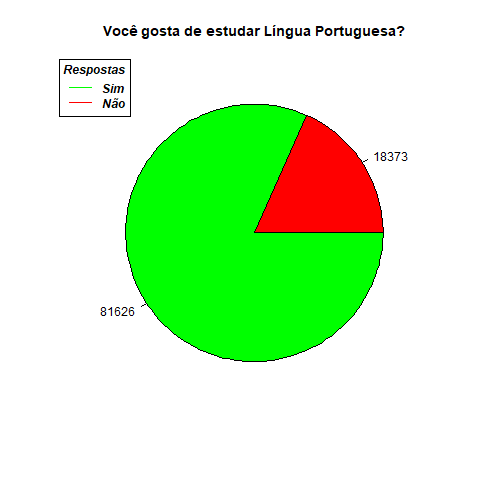
\includegraphics[width=0.7\linewidth]{gosta_lp.png}
    \centering
\end{figure}
Este gráfico mostra que a maioria dos estudantes do ensino básico afirmam gostar de estudar Língua Portuguesa, ou seja, \(\frac{81626}{99999} \approx 0.816\) ou 81.6 a cada 100 estudantes. \newline
Código-fonte:
\begin{lstlisting}
src <- read.table(file="sources\\DadosSaeb.csv", sep=";", header=TRUE)

gosta_lp <- table(src$"Voce.gosta.de.estudar.Lingua.Portuguesa.")

png(".\\graphs\\gosta_lp.png")
relatorio5 <- pie(
    as.numeric(gosta_lp),
    col=c("#ffa600", "#003f5c"),
    labels=as.numeric(gosta_lp),
    main="Voce gosta de estudar Lingua Portuguesa?",
)
legend(
    "topleft",
    legend=c("Sim", "Nao"),
    col=c("#003f5c", "#ffa600"),
    lty=1,
    cex=1,
    title="Respostas",
    text.font=4,
    bg="white"
)
dev.off()
\end{lstlisting}

\subsection{Boxplot para a variável "Nota Matemática"}
\begin{figure}[H]
    \includegraphics[width=0.7\linewidth]{box_mat.png}
    \centering
\end{figure}
Este gráfico mostra que a maioria das notas de Matemática ficam entre aproximadamente 220 e 270, com outliers acima de 375. \newline
Código-fonte: \newline
\begin{lstlisting}
# boxplot.r
box <- function(v, name, color, title) {
    png(paste("graphs\\box_", name, sep=""))
    boxplot(
        v,
        col=color,
        border="black",
        main=title
    )
    dev.off()
}

# boxplot_mat.r
source("scripts\\boxplot.r")

src <- read.table(file="sources\\DadosSaeb.csv", sep=";", header=TRUE)

nota_mat <- src$"Nota.Matematica"
box(nota_mat, "mat.png", "#003f5c", "Distribuicao da Nota de Matematica")
\end{lstlisting}

\subsection{Boxplot para a variável "Nota Português"}
\begin{figure}[H]
    \includegraphics[width=0.7\linewidth]{box_lp.png}
    \centering
\end{figure}
Este gráfico mostra que a maioria das notas de Português ficam entre aproximadamente 225 e 280, sem outliers. \newline
Código-fonte: \newline
\begin{lstlisting}
# boxplot.r
box <- function(v, name, color, title) {
    png(paste("graphs\\box_", name, sep=""))
    boxplot(
        v,
        col=color,
        border="black",
        main=title
    )
    dev.off()
}

# boxplot_lp.r
source("scripts\\boxplot.r")

src <- read.table(file="sources\\DadosSaeb.csv", sep=";", header=TRUE)

nota_lp <- src$"Nota.Portugues"
box(nota_lp, "lp.png", "#ffa600", "Distribuicao da Nota de Lingua Portuguesa")
\end{lstlisting}

\subsection{Histograma para a variável "Nota Matemática"}
\begin{figure}[H]
    \includegraphics[width=0.7\linewidth]{hist_mat.png}
    \centering
\end{figure}
Este gráfico mostra que as notas de Matemática estão distribuidas de forma homogênea, com alta concentração no centro. \newline
Código-fonte: \newline
\begin{lstlisting}
# hist.r
histogram <- function(v, name, color, title, ylim1) {
    png(paste("graphs\\hist_", name, sep=""))
    hist(
        as.numeric(v),
        col=color,
        main=title,
        xlab="Nota",
        ylab="Frequencia",
        xlim=c(100, 400),
        ylim=c(0, ylim1)
    )
    dev.off()
}

# hist_mat.r
source("scripts\\hist.r")

src <- read.table(file="sources\\DadosSaeb.csv", sep=";", header=TRUE)

nota_mat <- src$"Nota.Matematica"
histogram(nota_mat, "mat.png", "#003f5c", "Histograma da Nota de Matematica", 20000)
\end{lstlisting}

\subsection{Histograma para a variável "Nota Português"}
\begin{figure}[H]
    \includegraphics[width=0.7\linewidth]{hist_lp.png}
    \centering
\end{figure}
Este gráfico mostra que as notas de Português estão distribuidas de forma homogênea, com maior distribuição entre as classes. \newline
Código-fonte: \newline
\begin{lstlisting}
# hist.r
histogram <- function(v, name, color, title, ylim1) {
    png(paste("graphs\\hist_", name, sep=""))
    hist(
        as.numeric(v),
        col=color,
        main=title,
        xlab="Nota",
        ylab="Frequencia",
        xlim=c(100, 400),
        ylim=c(0, ylim1)
    )
    dev.off()
}

# hist_lp.r
source("scripts\\hist.r")

src <- read.table(file="sources\\DadosSaeb.csv", sep=";", header=TRUE)

nota_lp <- src$"Nota.Portugues"
histogram(nota_lp, "lp.png", "#ffa600", "Histograma da Nota de Portugues", 10000)
\end{lstlisting}

\newpage
\section{Referências bibliográficas}

\end{document}
